%%%%%%%%%%%%%%%%%%%%%%%%%%%%%%%%%%%%%%%%%%%%%%%%%%%%%%%%%%%%%%%%%%%%%%%%%%%%%%%%%%%%%%%%%%%%%%%%%%%%%%
%%%%%%%%%%%%%%%%%%%%%%%%%%%%%%%%%%%%%%%%%%%%%%%%%%%%%%%%%%%%%%%%%%%%%%%%%%%%%%%%%%%%%%%%%%%%%%%%%%%%%%
%%%%                                                                                       %%%%%%%%%%%
%%%% Plantilla de trabajo de titulación para la Carrera de Ingeniería en Construcción -UCM %%%%%%%%%%%
%%%% Elaborada por Carlos Palacios Rojas, Académico Dep Obras Civiles                      %%%%%%%%%%%
%%%% Versión 1.2.1 - 12 de septiembre de 2016                                              %%%%%%%%%%%
%%%% Las líneas que comienzan por "%" son comentarios y pueden ser eliminadas.             %%%%%%%%%%%
%%%% En caso de requerir más información del uso de los paquetes buscar en Internet.       %%%%%%%%%%%
%%%%                                                                                       %%%%%%%%%%%
%%%% Recomiendo el siguiente libro para consultas sobre Latex                              %%%%%%%%%%%
%%%% Mora, W., & Borbón, A. (2014). Edición de textos cientıficos con LATEX. 2da edición.  %%%%%%%%%%%
%%%%																					   %%%%%%%%%%%
%%%%%%%%%%%%%%%%%%%%%%%%%%%%%%%%%%%%%%%%%%%%%%%%%%%%%%%%%%%%%%%%%%%%%%%%%%%%%%%%%%%%%%%%%%%%%%%%%%%%%%
%%%%%%%%%%%%%%%%%%%%%%%%%%%%%%%%%%%%%%%%%%%%%%%%%%%%%%%%%%%%%%%%%%%%%%%%%%%%%%%%%%%%%%%%%%%%%%%%%%%%%%


\documentclass[10pt,letterpaper]{report}

	% Geometry: es para modificar los márgenes del documento
\usepackage[left=3cm, right=2.5cm, top=2.5cm, bottom=2.5cm]{geometry}
%% lipsum: para generar texto de ejemplo. Se puede eliminar una vez que se eliminen todos los \lipsum[] del documento.
\usepackage{lipsum}
% lscape: en caso de querer rotar una hoja, buscar información en internet en caso de ser requerido. 
\usepackage{lscape}
% inputenc: para que latex acepte caracteres latinos como los acentos y la letra ñ.
\usepackage[utf8]{inputenc}
% babel: para traducir los títulos que vienen originalmente en inglés. Ejemplo: Fecha, Chapter, Bibliography, Appendix, etc.
\usepackage[spanish,es-tabla]{babel}
% natbib: para poder citar utilizando paréntesis redondos con \citep{•} o sin parentesis con \cite{•}
\usepackage[round]{natbib}
\usepackage{float} % para usar [H] y obligar que las figuras o tablas aparezcan donde es requerido.
\usepackage[pdftex]{graphicx} % graphicx: para incorporar imágenes. Recordar que las imágenes 'gif' no son aceptadas por Latex, se sugiere utilizar formato png por su calidad, en segunda intantcia jpg.
\usepackage{parskip} % parskip: par no dejar sangrías e insertar espacios entre párrafos en su lugar.
\usepackage{amsmath} %paquete para escribir fórmulas matemáticas.
\usepackage{amsfonts}%paquete para escribir fórmulas matemáticas.
\usepackage{amssymb} %paquete para escribir fórmulas matemáticas.
\usepackage[usenames,dvipsnames,svgnames,table]{xcolor} %xcolor: para definir colores y dar color a tablas.

% hyperref: define opciones especiales para el documento PDF producido.
\usepackage[pdftex, bookmarksnumbered,  pagebackref, colorlinks=true, citecolor=DarkBlue, linkcolor=DarkBlue!30!Black, urlcolor=Black,bookmarksopen]{hyperref}

% El paquete fancyhdr es para definir opciones de encabezado y pié de página
% Según el formato existente a la fecha (agosto de 2015) esto no se considera
% Su utilización en este caso es para situar el número de página en la parte
% inferior derecha de la página.

\usepackage{fancyhdr} % activamos el paquete
	\pagestyle{fancy} % seleccionamos un estilo
	\lhead{} % texto izquierda de la cabecera
	\chead{} % texto centro de la cabecera
	\rhead{\textcolor[gray]{0.5}{\textit{\nouppercase \leftmark}}} % Nombre del capítulo. \nouppercase: uso de minúsculas
	\lfoot{} % texto izquierda del pie
	\cfoot{} % imagen centro del pie
	\rfoot{\textcolor[gray]{0.5}{\thepage}} % Número de página a la derecha, abajo
	\renewcommand{\headrulewidth}{0.2pt} % grosor de la línea de la cabecera

\fancypagestyle{detailed}{
    \fancyhf{} % clear all header and footers
    \fancyfoot[R]{\textcolor[gray]{0.5}{\thepage}}
	%\fancyhead{}    
    \renewcommand{\headrulewidth}{0pt}
 }
 
\usepackage{etoolbox}
\patchcmd{\chapter}{\thispagestyle{plain}}{\thispagestyle{detailed}}{}{}

%times: para uar letra tipo Times New Roman
\usepackage{times}

%separación entre líneas (1.2 espacios). En word es interlineado exacto a 12 pts
\renewcommand{\baselinestretch}{1.2} 

\usepackage{titlesec} % para poder modificar los títulos

% Para la numeración de tablas y figuras.
\renewcommand\thefigure{\arabic{section}.\arabic{figure}} % Genera numeración X.Y
\renewcommand\thetable{\arabic{section}.\arabic{table}} % Genera numeración X.Y
\numberwithin{figure}{section} %Hace que la primera figura de cada sección X sea X.1
\numberwithin{table}{section} %Hace que la primera tabla de cada sección X sea X

\usepackage{booktabs} % Para trabajar con opciones especiales de tablas.
\usepackage{caption}


% El índice de tablas e imágenes se superpone el texto al número de la figura o tabla.
% Esta configuración arregla dicho problema, modificar el 3.0 de ser necesario.
\usepackage{tocloft}
\addtolength{\cftfignumwidth}{3.0em}
\renewcommand{\cftfigpresnum}{\figurename\ }
\addtolength{\cfttabnumwidth}{3.0em}
\renewcommand{\cfttabpresnum}{\tablename\ }



				
\begin{document}

	\logo{
\includegraphics[scale=0.15]{imagenes/logoUniversidad}}
\begin{frame}[plain]

\begin{columns}

	\begin{column}{5cm}
	
\includegraphics[scale=0.2]{imagenes/logoICO}
	\end{column}

	\begin{column}{5cm}
	\begin{flushright}
	
\includegraphics[scale=0.3]{imagenes/logoUCM}
	\end{flushright}
	\end{column}

\end{columns}
\maketitle

\end{frame}
%%-------------------------------------------------------------------------------------

 \begin{frame}{Contenido}
 \tableofcontents
 \end{frame}

%%-------------------------------------------------------------------------------------
	
\chapter*{Dedicatoria}

Dedico este trabajo a las futuras generaciones para que recuerden que siempre deben creer en si mismos y en sus sueños.


%--------------------------------------------------------
\chapter*{Agradecimientos}

Agradecer a mi madre Ana María por todo el esfuerzo, amor y ternura que entregó siempre a todos sus hijos, a mi padre Pedro Juan por haber estado ahí siempre con nosotros enseñandome cosas que un hombre necesita saber para ser un hombre de bien, a mi hermana mayor Fiorella porque con el ejemplo siempre me oriento a tomar buenas decisiones, a mi hermana Kerly porque me enseñó que un buen corazón siempre obra bien con todas las formas de vida, a mi hermano Jimmy porque es mi amigo con el que he pasado muchas horas divirtiendonos y aprendiendo juntos; a mi profesor Raúl Vargas Roncal que fue un consejero y amigo cuando más lo necesité en mis épocas de estudios universitarios, a mi profesor William Chauca con el que pasaba tardes en la universidad conversando y me orientaba como un amigo, a mi profesor Emanuel Guzman que siempre fue un mentor y amigo con el que conversabamos sobre la vida, él también me enseñaba sobre el modelamiento numérico y el océano para poder crecer como profesional, a la Dra. Elisa Armijos porque ella ha sido una gran amiga que con sus consejos me orientaba para hacer posible este trabajo de investigación, siempre estuvo presente cuando la necesité y me invitaba a seguir motivado, a mis amigos de Makerlab Perú porque sábado a sábado he crecido con ellos compartiendo experiencias, a mi compañero Renzo porque vivíamos juntos la experiencia de ser tesistas en una institución tan prestigiosa, al Instituto Geofísico del Perú por permitirme ingresar a un mundo nuevo y hacer posible mi pasión, el desarrollar tecnología fué algo que siempre me despertó y gracias a ellos esto ha sido posible.




%--------------------------------------------------------

\chapter*{Resumen}

La importancia del estudio de los ríos en el Perú en la decada del 2010 viene porque en los últimos años se ha visto muy importante el estudio de las precipitaciones en las zonas de alta montaña debido a los efectos del cambio climático, al ubicarnos muy cerca al Ecuador en la zona norte del país se ven muy vunerables ante las grandes crecidas de los ríos donde traen mucho material flotante que es perjudicial para las zonas bajas donde vive la población; por ello la comprensión y la toma de decisiones anticipada es estratégico para que las comunidades no se vean vulneradas; en épocas de máximas avenidas no se pueden hacer mediciones con los equipos por ser muy riesgosos para el personal y para estos ya podrían ser arrastrados y perderse, este software hidro-sedimentario gestionará una base de datos de caudales líquidos y sólidos permitiendo a los científicos e ingenieros analizar el comportamiento del río.



\vspace{1cm}
\textbf{\textit{Palabras claves}}--- 
Cambio climático, máximas avenidas, software hidro-sedimentario, bases de datos, caudales líquidos y sólidos.





























% No borrar esta sección...

\newpage
%--------------------------------------------------------
%Aquí se genera el índice de la tesis (\tableofcontents)
\tableofcontents
\newpage
%--------------------------------------------------------
%Aquí se genera el índice de tablas (\listoftables)
\listoftables

%--------------------------------------------------------
%Aquí se genera el índice de imágenes (\listoffigures)
\listoffigures

%--------------------------------------------------------
%También es posible realizar índice de ecuaciones, buscar en google por "indice de ecuaciones latex"

%Aquí comienza a numerarse las páginas con números arabigos.
\pagenumbering{arabic}
 % Dedicatoria, agradecimientos y resumen

\chapter{Introducción}

Un paquete hidro-sedimentario ayuda a la toma de mejores decisiones en la gestión de los recursos  hídricos consolidando una base de datos que permita recopilar a lo largo de los años los datos de hidráulica y de sedimentos. Esta base ayuda a poder analizar el comportamiento de los ríos, determinar las épocas de máximas crecidas y secas.
Contar con una base igualmente permite tener un mejor acceso para un mayor público científico y técnico.
Una de las ventajas de tener una herramienta con paquetes libres es el acceso, la continua actualización y evitar la pirateria.
El paquete que se desea proponer estará alojado en una plataforma web que permita colocar los datos en una nube, sin embargo el primer paso es hacer esto posible en un localhost que brinde posibilidades de acceso desde centros de estudio, centros de investigación o incluso para el sector privado; nuestra propuesta pretende beneficiar a todos ellos con este motivo se pone bajo la licencia GPL ( General Public License).

Se busca desarrollar un software que junte la parte hidráulica y sedimentológica porque con ello se podrá realizar el ánalisis de los flujos sedimentarios. Hoy en el mercado son muy pocos los productos que cumplan con estas tareas y las que hay tienen limitaciones porque exigen al usuario depender de otros softwares privativos. El Observatorio ORE-HYBAN cuenta con el software HydroMESAD que es un programa en su versión beta que cumple con tener una base de datos y con estos realizar relaciones entre si. Sin embargo El HydroMESAD presenta un estado de dependencia al software privativo Acces - Microsoft Office presentando dificultades tanto por costo del producto como por las actualizaciones ya que estas no se viene actulizando al mismo ritmo que este último.

Este trabajo tiene como objetivo crear un software amigable e intuitivo para el usuario y que a la vez logre contar con una base de datos, interfaz gráfica de usuario, relacionar variables hidráulicas e de sedimentos.

Un software en código abierto y abre las posibilidades de trabajar con más desarrolladores en el mundo a través de herramientas de control de versiones. Para construir un software hay muchos caminos, sea a partir de código puro o a través de entornos de trabajo para su desarrollo. 

	\section{Descripción del problema}
	
	En países en vías de desarrollo como el nuestro muchas veces se hacen malas practicas de piratería informática en herramientas de software para la ingeniería, el estudio de los ríos es de mucho interés para la sociedad ya que de la toma de decisiones que hagan las autoridades va a repercutir directamente a la población; se necesita que estas herramientas tecnológicas sean de acceso común para todo el mundo y sea mantenido por una comunidad de desarrolladores aportando mejoras o modificaciones, si bien es cierto hay cálculos que se pueden desarrollar a partir de un programa de computadora muchas veces encontramos personas que ocupan cargos en empresas o en instituciones públicas que no cuentan de momento con estas competencias y no se puede analizar lo que viene ocurriendo con las fuentes hídricas de las que ellos son responsables.

	
		\subsection{Problema específico}
			La hidrología requiere de un estudio para su entendimiento y en el desarrollo de estas herramientas tecnológicas se ha visto muy pocos profesionales en nuestro país que hagan esto posible, contando con una geografía tan accidentada como la nuestra necesitamos poder tener herramientas hechas para nuestras necesidades específicas por ello la importancia de que un mecánico de fluídos para que haga esto algo posible.
			Sub sección de la \textit{Descripción del problema}
 
	\section{Objetivo general}
	
	\begin{itemize}
	\item Crear un software hidrosedimentario con interfaz gráfica de usuario.
	\item Brindar un producto que ayude a los científicos e ingenieros que trabajan con fluídos geofísicos.
	\item Entregar un producto open-source para la comunidad científica internacional.
	\end{itemize}

	\section{Objetivos específicos}

	Los objetivos específicos que contribuirán a desarrollar el \textit{objetivo general} del trabajo son los siguientes:

	\begin{itemize}
		\item Crear una lectura de archivos de caudales.
		\item Crear un formulario para insertar los datos de las muestras se sedimentos.
		\item Crear una base de datos.
		\item Gráficar la sección del río para visualizar las cotas de fondo y los valores de sedimentos en suspensión.
	\end{itemize}

	\section{Contribución del trabajo de titulación}

El presente trabajo da las posibilidades de poder estudiar mejor el cambio climático por la erosión que se presentan por las intensas precipitaciones aguas arriba ya que por ello vienen más sedimentos, el resultado de esta investigación hace posible que futuros especialistas técnicos puedan caracterizar mejor los perfiles de velocidad y sedimentos.

\chapter{Marco teórico}	
Para crear un software con interfaz gráfica de usuario se requiere de la comprensión de la programación orientada a objetos, conocimientos en bases de datos y en sistemas de control de versiones.
\section{Lenguaje de programación Python}
El lenguaje de programación Python es open-source lo que significa que el usuario no necesita pagar una licencia para su uso, este lenguaje ha sido inventado por Guido van Rossum en el año 1991 inspirado en el grupo humorita de la época Monty Python.

Python es un lenguaje multipropósito, a la fecha ya se encuentra en su versión 3, a diferencia de otros lenguajes de programación este se caracteriza por su facilidad para escribir ya que unicamente depende de la identación como requisito para que sea funcional, es decir no como en otros lenguajes que necesitas señalar ";" para terminal una sentencia de línea.

Python también es un lenguaje orientado a objetos.

Es un lenguaje de código abierto que nació en 1991 gracias a Guido Van Rossun, el nombre viene en memoria del grupo músical Monty Python.

La Python Software Foundation es la organización sin animos de lucro que viene promoviendo, protegiendo y desarrollando mejoras al lenguaje Python.

\begin{itemize}
\item Ventajas
	\begin{itemize}
	\item Una gran comunidad en el mundo.
	\item Es un lenguaje de c\'odigo abierto.
	\item Una curva de aprendizaje corta.
	\item Es un lenguaje multiprop\'osito.
	\item Se puede usar como pegamento con otros lenguajes de programaci\'on evitando as\'i los famosos cuellos de botella, por ejemplo se podr\'ia encapsular scripts en lenguajes C o Fortran y as\'i dejar corriendo de ser necesario en servidores para casos como la modelaci\'on num\'erica.
	\item La implementaci\'on de un programa es muy r\'apido comparado a hacer el mismo programa de computadora con otro lenguaje.
	\item Es multiplataforma por lo que corre en sistemas operativos Windows, Mac Os X y GNU/Linux.
	\item Se pueden crear entornos virtuales para que se trabaje de manera independiente con distintas versiones de Python y no ocurra conflictos de librer\'ias.
	\end{itemize}
\item Desventajas
	\begin{itemize}
	\item Es lento si se compara su velocidad de c\'alculo con Fortran o C sin hacer ningun artificio.
	\item Existen conflictos con las librer\'ias si se usan versiones del lenguaje distintos.
	\end{itemize}
\end{itemize}
\section{Bases de datos}

Las bases de datos nos permiten trabajar con grandes volumenes de datos evitando que el usuario pueda cometer errores como el de eliminar un registro por error y si darse cuenta guardar los cambios; si nos referimos como tal una base de datos se caracteriza porque esta es intangible para el usuario, él no podrá manipularlo directamente, las bases de datos hay de dos tipos que son las relacionales y no relaciones las, las relacionales son más seguras y un poco más lentas mientras que las no relacionales son inversar a lo anterior.

Para trabajar con bases de datos tenemos como principales lenguajes de consulta a:

\begin{itemize}
\item MySql
\item SQLite
\item MongoDB
\item Postgres
\end{itemize}

\section{Git}
	
	\cite{solminihac2005} 
	
	%ejemplo de cita 'En el texto' sin parentesis, para citar con parentesis usar \citep{}


\chapter{Metodología}


	\section{Título primera sección capítulo}
	
		% Para trabajar con tablas sugiero utilizar Macro Excel2Latex (ver carpeta útiles)
		% La tabla siguiente tiene dos columnas y se indican con '{l c}'

		\begin{table}[h]
			\caption{Título de la tabla.} 
			\begin{center} % tabla centrada en el texto
				\begin{tabular}{l c} %l -> left, c -> center, r -> right
					\hline % línea horizontal
					\hline 
					Título 1 & Título 2 \\  % Fila de encabezados 
					\hline
					Cuadro 1 & Cuadro 2 \\  % (\\ indica el final de la línea)
					Cuadro 3 & Cuadro 4 \\
					\hline
					\hline
				\end{tabular}
			\label{tablaUno}
	     % label: etiqueta tabla, sirve para ref. cruzadas, ver video: 
    	 % https://www.youtube.com/watch?v=ldU2mEWAeh4

			\end{center}
		\end{table}

		La Tabla \ref{tablaUno} ejemplifica el uso de tablas en \LaTeX. \citep{solminihac2005} % ej. de cita entre paréntesis.


	\subsection{Subtítulo.}


		\begin{figure}[h]
			\centering
			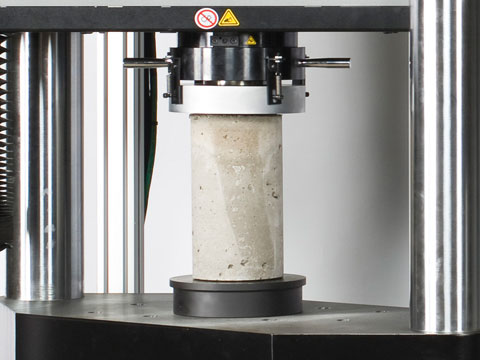
\includegraphics[scale=0.5]{imagenes/ASTM_C39_image1.jpg}
			\caption{Probeta hormigón (Autor, año)}
			\label{probetaHormigon} 
			% Label: es para realizar referencias cruzadas, 
			% notar que se escribe todo junto y sin acentos.
		\end{figure}

	La Figura \ref{probetaHormigon} Muestra ... (Explicar las figuras. Notar que la figura fue
	citada con referencia cruzada y la numeración es automática) 
	
	%% Ver video referencias cruzadas: https://www.youtube.com/watch?v=ldU2mEWAeh4


\chapter{Resultados.} 

	
	\section{Ejemplo de titulo 2.}
		
		\subsection{Ejemplo de titulo 3.}
			
			\subsubsection{Ejemplo de titulo 4 (no numerado).}

				\paragraph{Ejemplo de título 5:}

								
	\section{Discusión de resultados.}


\chapter{Conclusiones}





%%%%%%%%%%%%%%%%%%%%%%%%%%%%%%%%%%%%%%%%%%%%%%%%%%%%%%%%%%%%%%%%%%%%%%%%%%%%%%%%%%%%%%%%%%%%%%%%%
%%%%%%%%%%%%%%%%%%%%%%%%%%%%%%%%%%%% Bibliografía %%%%%%%%%%%%%%%%%%%%%%%%%%%%%%%%%%%%%%%%%%%%%%%
%%%%%%%%%%%%%%%%%%%%%%%%%%%%%%%%%%%%%%%%%%%%%%%%%%%%%%%%%%%%%%%%%%%%%%%%%%%%%%%%%%%%%%%%%%%%%%%%%
	
	% Para aprender a usar la bibliografía ver el siguiente video:
 	% https://www.youtube.com/watch?v=MnL5dI41IOA

	% No modificar esta sección
 
	\renewcommand{\refname}{Bibliografía} % Bibliografía en español
	\addcontentsline{toc}{chapter}{Bibliografía} % Agrega la bibliografía al Índice.
	\bibliographystyle{apalike} % formato APA 

	\bibliography{perifericos/bibliografia} 


%%%%%%%%%%%%%%%%%%%%%%%%%%%%%%%%%%%%%%%%%%%%%%%%%%%%%%%%%%%%%%%%%%%%%%%%%%%%%%%%%%%%%%%%%%%%%%%%%
%%%%%%%%%%%%%%%%%%%%%%%%%%%%%%%%%%%% Anexos o apéndices %%%%%%%%%%%%%%%%%%%%%%%%%%%%%%%%%%%%%%%%%
%%%%%%%%%%%%%%%%%%%%%%%%%%%%%%%%%%%%%%%%%%%%%%%%%%%%%%%%%%%%%%%%%%%%%%%%%%%%%%%%%%%%%%%%%%%%%%%%%


	% El siguiente archivo conntiene los apéndices
	% Está en un archivo diferente para que el presente archivo sea menos extenso.
	% En caso de no existir anexos simplemente eliminar o anteponer '%'
	
\appendix

\chapter{Ejemplo de apéndice o anexo}

\section{Sub título primer apéndice o anexo}



\subsection{Sub sección del primer apéndice o anexo}




\end{document}